\documentclass[sigconf,nonacm]{acmart}
%% Standalone Paper 1 of 2 — GNN contagion prediction. Overleaf- and TinyTeX-ready.
\usepackage{booktabs}
\usepackage{graphicx}
\usepackage{amsmath}
\let\Bbbk\relax
\usepackage{amssymb}
\usepackage{multirow}
\settopmatter{printacmref=false}
\renewcommand\footnotetextcopyrightpermission[1]{}
\pagestyle{plain}

\begin{document}

\title{Predicting Cross-Asset Stablecoin Contagion with Temporal Graph
Neural Networks}

\author{Anonymous Author(s)}
\affiliation{\institution{Columbia University, MAFN}\city{New York}\country{USA}}

\begin{abstract}
On 10 March 2023, the stablecoin USDC---a token designed to always trade at exactly one US
dollar---fell to \$0.88 after its issuer disclosed that \$3.3B of its cash reserves were trapped
at the failed Silicon Valley Bank. Within hours, \emph{other} dollar stablecoins wobbled too.
This paper asks a concrete, operational question: when one stablecoin breaks its dollar peg,
\emph{which other stablecoins will follow, and how soon?} We treat this as a prediction problem
on a network that evolves through time, using real minute-by-minute price data from two large
exchanges across seven crisis episodes in 2022--2023. We compare a full ladder of models---from
simple baselines to gradient-boosted trees to temporal graph neural networks (GNNs)---under an
evaluation protocol carefully designed to prevent the model from ``cheating'' by seeing
overlapping crises. Two findings stand out. First, contagion is essentially \emph{unpredictable}
at horizons of a few hours, but becomes predictable at a one-day horizon, where a graph-attention
network (GAT) beats every non-graph model by $0.18$ in precision--recall AUC. Second, an ablation
that deletes the network's edges shows that this advantage comes specifically from the
\emph{relationships between stablecoins}, not merely from a more flexible model. We deliver an
interpretable ranking of the most systemically central venues in each crisis, designed as the
input to downstream risk and policy analysis.
\end{abstract}

\keywords{stablecoins, financial contagion, temporal graph neural networks, graph attention,
systemic risk, leakage-safe evaluation}

\maketitle

\section{Introduction}

\subsection{What is a stablecoin, and what is a depeg?}
A \emph{stablecoin} is a cryptocurrency token engineered to hold a constant value, almost always
one US dollar. Users treat \$1 of a stablecoin as interchangeable with \$1 of cash, which is why
stablecoins now settle trillions of dollars of transactions and underpin much of decentralized
finance. The largest fiat-backed stablecoins (USDC, USDT, formerly BUSD) promise that every token
is backed one-for-one by cash and short-term government debt; crypto-collateralized coins (DAI,
FRAX) are instead backed by a basket of other crypto assets, often \emph{including other
stablecoins}.

When a stablecoin's market price moves away from \$1, it is said to \emph{depeg}. A depeg is the
crypto analogue of a bank run: holders fear the token is no longer fully backed and rush to sell
or redeem it, pushing the price further down. Because regulators now treat stablecoins as
systemically important---both the US GENIUS Act and the EU's MiCA regulation make reserve adequacy
and contagion containment central concerns~\cite{genius2025,mica2023}---understanding how one
depeg spreads to others is a question with direct policy stakes.

\subsection{A concrete example: the SVB weekend}
On the weekend of 10--12 March 2023, Silicon Valley Bank failed. Circle, the issuer of USDC,
disclosed that \$3.3B of the cash backing USDC was stuck at SVB. The market could not tell whether
that money would be recovered, and USDC---supposedly worth exactly \$1---traded as low as
\$0.88. Crucially, the panic did not stay contained. \textbf{DAI} fell too, because a large share
of DAI's collateral was \emph{itself} USDC; \textbf{FRAX}, roughly 90\% USDC-backed, also dropped;
and even unrelated coins such as \textbf{TUSD} and \textbf{Pax Dollar (USDP)} wobbled as traders
fled stablecoins indiscriminately. Figure~\ref{fig:depeg} shows the real minute-level paths.
This is \emph{contagion}: a shock to one node of a financial network propagating to others.

\subsection{The prediction problem and our contributions}
We ask: given the state of the stablecoin market at time $t$, can we predict which currently
healthy stablecoins will depeg within a horizon $\Delta$? This is a forecasting problem on a
\emph{temporal graph}---a network whose nodes are trading venues, whose edges capture which venues
move together and in what order, and whose structure changes minute by minute. Graph neural
networks are the natural model class for learning on such structured, evolving data, and have
recently been applied to related on-chain prediction tasks such as liquidity-pool bridge swaps on
Uniswap~\cite{zhou2025bridge}. Our contributions are:
\begin{enumerate}
\item A contagion predictor trained on \textbf{real} multi-venue, minute-level data, evaluated
under a \textbf{leakage-safe} protocol that we show is essential (\S\ref{sec:data}).
\item A \textbf{lead-time} finding: contagion is unpredictable at hours but predictable at a day,
established with metrics that are not inflated by class imbalance (\S\ref{sec:results}).
\item An \textbf{ablation} that isolates how much of the model's skill comes from the network
structure itself, and shows the answer is attention-specific (\S\ref{sec:results}).
\item An interpretable, exportable \textbf{hub ranking} that names the most central venues in each
crisis (\S\ref{sec:interp}).
\end{enumerate}

\begin{figure}[t]
\centering

\includegraphics[width=\columnwidth]{figures/01_depeg_paths.png}
\caption{Real 1-minute prices during the USDC/SVB crisis (Binance and Coinbase). USDC and several
peers fall to \$0.86--0.95 on 11 March 2023 and recover by the 13th. The spread of the drop across
\emph{different} coins is the contagion this paper predicts.}
\label{fig:depeg}
\end{figure}

\section{Background and related work}
\paragraph{Graph neural networks in one paragraph.} A graph neural network learns a representation
for each node by repeatedly mixing the node's own features with those of its neighbours---``message
passing.'' \textbf{GraphSAGE}~\cite{hamilton2017graphsage} averages neighbour information;
\textbf{graph attention networks (GAT)}~\cite{velickovic2018gat} instead \emph{learn how much
weight} to give each neighbour, which matters when some relationships are far more informative
than others. A \emph{temporal} graph applies this at each time step on a network that itself
changes over time.

\paragraph{Prior work.} GNNs have been used to predict on-chain events such as cross-pool bridge
swaps in Uniswap v3~\cite{zhou2025bridge}, but evaluate \emph{prediction}, not which nodes
\emph{cause} propagation. Tree ensembles such as XGBoost~\cite{chen2016xgboost} are the strong
tabular baseline we must beat to justify a graph model. We follow this literature in framing
contagion as a temporal node-classification task, and depart from it by (i) working cross-asset on
the deepest centralized venues, where minute-level data is cleanest, and (ii) treating leakage
control as a first-class design constraint.

\section{Data and task formulation}\label{sec:data}
\paragraph{Data.} We collect real 1-minute open/high/low/close/volume bars from
\textbf{Binance} (for USDC, TUSD, USDP, FRAX, BUSD, FDUSD, and the failed algorithmic coin UST,
all quoted against USDT) and \textbf{Coinbase} (for DAI and USDT, quoted against the US dollar).
Because Binance prices are quoted in USDT rather than dollars, we multiply them by the Coinbase
USDT/USD price so that a wobble in USDT itself is not hidden by the choice of quote currency. We
assemble seven historical crisis episodes: the Terra/UST collapse and the secondary USDT scare
(May 2022), the FTX-driven DAI stress (Nov 2022), the regulatory BUSD wind-down (Feb 2023), the
USDC and FRAX SVB depegs (Mar 2023), and the 2018 USDT scare.

\paragraph{Nodes, samples, and labels.} A \emph{node} is an (asset, venue) pair, e.g.\ ``USDC on
Binance.'' We sample the market once per hour; each (hourly snapshot, node) pair is one training
example. The \emph{label} is contagion \emph{onset}: node $j$ enters a \emph{new} sustained stress
period---its price more than an asset-class-specific threshold (25 basis points for fiat-backed,
75 for crypto-backed) away from \$1 for at least ten consecutive minutes---within the next
$\Delta$ minutes, given that it was calm at time $t$. The coin that triggered the episode (the
``origin'') is excluded, because we want to predict \emph{spread}, not the initial shock. We use
four horizons: 30 minutes, 1 hour, 4 hours, and 24 hours.

\paragraph{Why leakage control is the crux.} The FRAX/SVB and USDC/SVB episodes occupy the
\emph{same} calendar window of March 2023. If one is placed in the training set and the other in
the test set, a model can memorize the idiosyncratic market conditions of that weekend and appear
near-perfect---we observed XGBoost reaching a PR-AUC of $1.0$, an obvious artifact. We therefore
group same-window episodes into \emph{clusters} and never split a cluster across train and test.
We report two protocols: a held-out SVB cluster, and leave-one-cluster-out (LOCO), in which each
cluster takes a turn as the test set. This single discipline is what separates an honest result
from a misleading one.

\section{Models}
We evaluate a \emph{ladder} of models on identical samples, from simplest to most expressive:
(1) \emph{majority} and \emph{persistence} baselines; (2) \emph{logistic regression} and
\emph{XGBoost}~\cite{chen2016xgboost} on each node's own features; (3) a \emph{GRU} recurrent
network on per-node feature sequences; and (4) two GNNs, \emph{GraphSAGE} and \emph{GAT}, on the
temporal graph. Node features are standard market-microstructure signals---price deviation from
\$1, realized volatility over 1 and 24 hours, trading volume, Amihud illiquidity, Kyle's
$\lambda$ (price impact of order flow), and the speed of mean-reversion (the Ornstein--Uhlenbeck
half-life)---plus short lags. Edges are built from a 6-hour rolling \emph{directed lead--lag}
graph: we connect two venues if their returns are correlated, and orient the edge from the
\emph{leader} (the one that moves first) to the \emph{follower}. The GNNs predict onset for every
active, non-origin node at each snapshot, trained with class-weighted loss (positives are rare)
and early stopping. Reporting a full ladder lets us attribute any gain to the right cause: the
sequence model isolates the value of temporal dynamics, and the GNNs isolate the value of the
network.

\section{Results}\label{sec:results}
\paragraph{The right yardstick.} Depeg onset is a rare event, so we use precision--recall AUC
(PR-AUC) rather than accuracy. But PR-AUC mechanically rises as the base rate rises (and our base
rate grows from 2.6\% at 30 minutes to 29\% at 24 hours), so comparing raw PR-AUC \emph{across}
horizons is misleading. We therefore also report ROC-AUC, which is invariant to the base rate, and
PR-AUC \emph{lift} (PR-AUC minus the base rate). A model with no skill scores ROC-AUC $0.5$ and
lift $0$.

\paragraph{Lead-time.} Figure~\ref{fig:leadtime} tells the central story. At horizons of four
hours or less, \emph{no} model exceeds chance: short-term contagion onset is not predictable from
price microstructure. At 24 hours, only the graph models clear ROC-AUC $0.5$, with GraphSAGE
reaching $0.65$. Contagion onset in this market is a \emph{day-scale} phenomenon; the hour-scale
negative result is real and honestly scopes the claim.

\begin{figure}[t]
\centering

\includegraphics[width=\columnwidth]{figures/02_leadtime.png}
\caption{Lead-time. \emph{Left:} ranking skill (ROC-AUC) versus horizon---only the graph models
beat chance ($0.5$, dashed) at 24h. \emph{Right:} precision lift over the base rate. Per-node
tabular models stay near zero skill.}
\label{fig:leadtime}
\end{figure}

\paragraph{Headline (averaged over five seeds).} On the held-out SVB cluster at 24 hours, GAT
attains PR-AUC $0.447 \pm 0.016$, a margin of $\mathbf{+0.175 \pm 0.016}$ over XGBoost, which sits
exactly at the base rate of $0.29$. We stress the multi-seed reporting: a single unlucky random
seed gives GAT only $0.29$, so a single run would have understated the effect. In the harder LOCO
protocol the per-fold margins shrink but stay positive (Fig.~\ref{fig:loco}); they survive
dropping the degenerate USDT-2018 fold, which contains a single positive example (GAT remains
$+0.083$ over XGBoost on the remaining folds).

\begin{figure}[t]
\centering
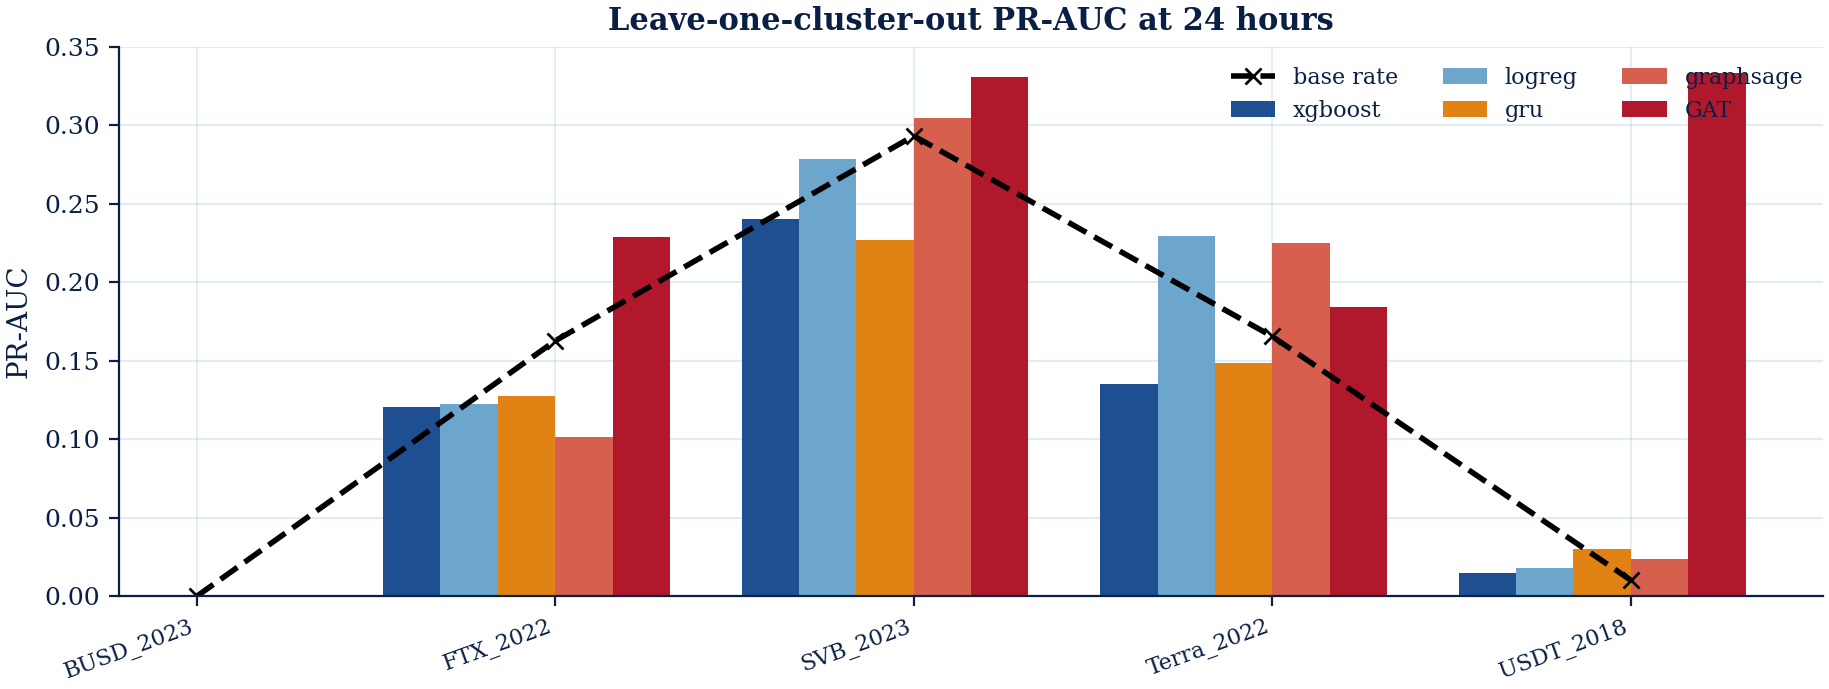
\includegraphics[width=\columnwidth]{figures/03_loeo_bars.png}
\caption{Leave-one-cluster-out PR-AUC at 24h. Graph models (GAT in dark red) lead the tabular
baseline on the contagion-bearing folds; the single-positive USDT-2018 fold is a high-variance
outlier we report but do not lean on.}
\label{fig:loco}
\end{figure}

\paragraph{Ablation: is it the graph or the model?} A skeptic will ask whether the GNN wins simply
because it is a more flexible neural network, not because it uses the \emph{network}. We answer by
re-running the GNNs with all edges deleted---turning each into a per-node neural network with no
message passing---and comparing to the same architecture with the real edges (Table~\ref{tab:ablation}).
The jump from XGBoost ($0.271$) to the edge-free GNNs ($0.35$--$0.39$) is the value of the neural
architecture. The further jump to the edge-equipped models is the value of the \emph{graph}: the
directed lead--lag edges add $\mathbf{+0.100}$ PR-AUC for GAT but only $+0.009$ for GraphSAGE. The
cross-asset relationships therefore carry genuine contagion signal, and \emph{graph attention}---
the ability to weight some neighbours more than others---is what exploits it. This both justifies
the graph model and explains why attention, specifically, is the winner.

\begin{table}[t]
\caption{Graph ablation, held-out SVB cluster @ 24h, mean of 5 seeds. ``Graph contribution'' is
real-edges minus no-edges, holding the architecture fixed.}
\label{tab:ablation}
\begin{tabular}{lrr}
\toprule
Model rung & PR-AUC & graph contribution \\
\midrule
node-only (XGBoost) & 0.271 & --- \\
GraphSAGE, no edges & 0.392 & \multirow{2}{*}{$+0.009$} \\
GraphSAGE, real edges & 0.401 & \\
GAT, no edges & 0.347 & \multirow{2}{*}{$\mathbf{+0.100}$} \\
GAT, real edges & \textbf{0.447} & \\
\bottomrule
\end{tabular}
\end{table}

\section{Interpretation and the exported hub ranking}\label{sec:interp}
Beyond a prediction, a risk team wants to know \emph{which signals matter} and \emph{which venues
are central}. The strongest individual predictors (XGBoost feature importance;
Fig.~\ref{fig:features}) are the speed of mean-reversion (OU half-life) and recent 24-hour
volatility---intuitively, a coin that is reverting slowly and trading turbulently is fragile.

We summarize each crisis with an interpretable \emph{hub ranking} that combines three ingredients:
how much a node influences the GNN's predictions (measured by occlusion---how much predictions
change when we zero out that node, a perturbation-based and software-version-robust alternative to
GNNExplainer-style masks~\cite{ying2019gnnexplainer}); its graph betweenness centrality; and a
\emph{propagator label} computed directly from raw prices (so it is not circular with the model).
For the USDC/SVB crisis the top-ranked hub is \textbf{BUSD} (Fig.~\ref{fig:hubmap}). We deliberately
stop at \emph{ranking}. Whether a highly ranked, highly central hub is actually \emph{causally}
responsible for spreading contagion---and what happens to a regulator who acts on a merely
correlational ranking---is a distinct question that requires an intervenable model, which we
address in a companion study that consumes exactly this exported ranking.

\begin{figure}[t]
\centering
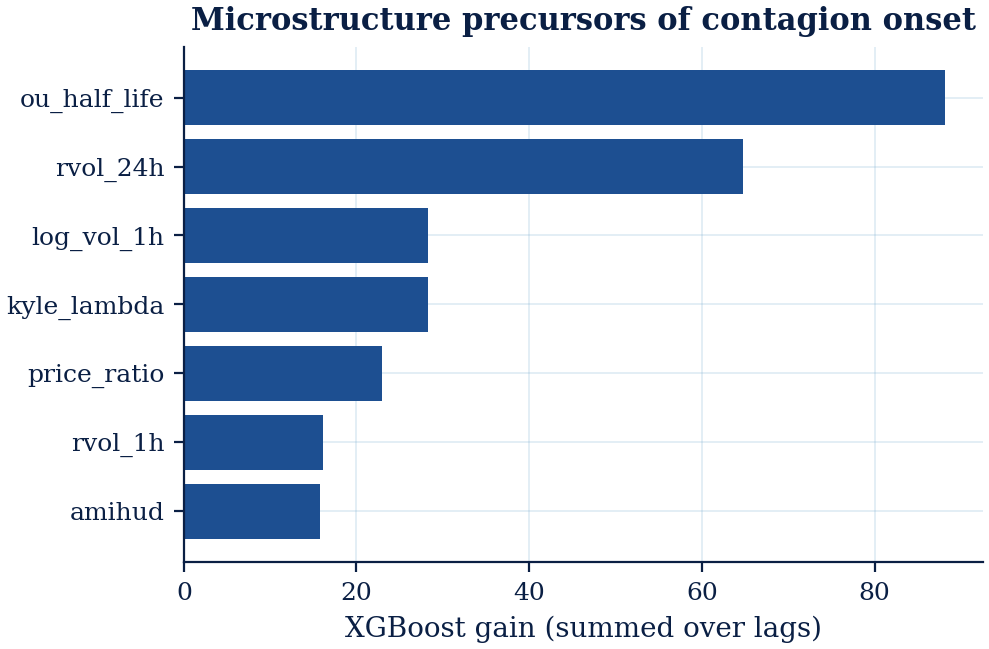
\includegraphics[width=\columnwidth]{figures/04_features.png}
\caption{Which signals predict contagion onset (XGBoost gain, summed over lags). Mean-reversion
speed and recent volatility dominate.}
\label{fig:features}
\end{figure}

\begin{figure}[t]
\centering
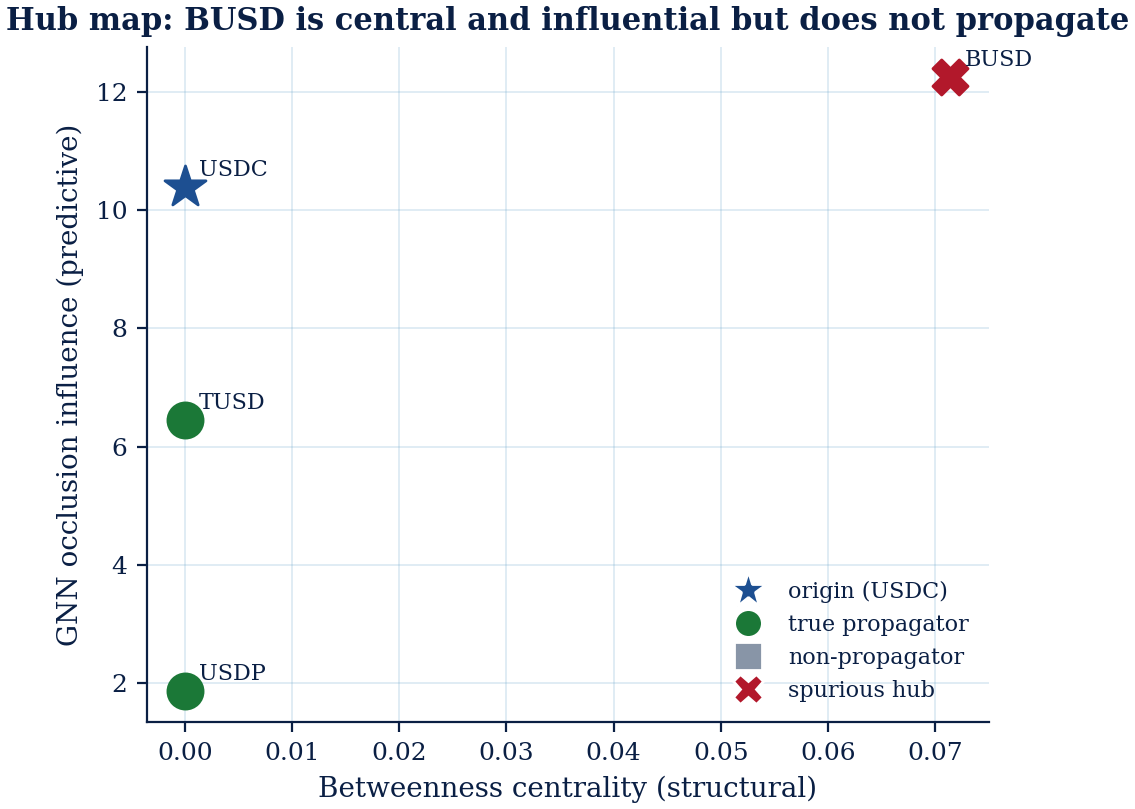
\includegraphics[width=\columnwidth]{figures/05_hub_map.png}
\caption{Exported hub map for USDC/SVB: graph betweenness (x) versus GNN influence (y), with the
origin (USDC) marked separately. The top-ranked hub is the actionable output handed to causal
analysis.}
\label{fig:hubmap}
\end{figure}

\section{Limitations}
We study seven episodes on the cleanly fetchable cross-asset universe of two large exchanges; two
episodes are too sparse (a single active venue, almost no contagion) to carry signal. The
lead--lag edges can over-credit thinly traded coins that merely appear to ``lead'' because of
noise. Short-horizon onset is genuinely unpredictable in our data, and we report this rather than
hide it. Finally, the hub ranking is correlational by construction; establishing causation is out
of scope here and is the subject of companion work.

\section{Conclusion}
On real multi-venue data, day-scale stablecoin contagion is predictable, and a graph-attention
network adds real, \emph{edge-borne} signal---an extra $0.10$ in PR-AUC over the same model
without the network---while hour-scale onset is not predictable at all. The method produces an
interpretable, exportable ranking of systemically central venues. How to act on that ranking
safely depends on whether its hubs are causal, the question we turn to next.

\paragraph{Reproducibility.} Every number above is produced by committed scripts; a single
\texttt{reproduce.sh} regenerates all datasets, results, figures, and the hub export end-to-end.

\bibliographystyle{ACM-Reference-Format}
\bibliography{references}

\end{document}
